\begin{figure}[!htb]
    % \centering
    \Subfigure[0.49]{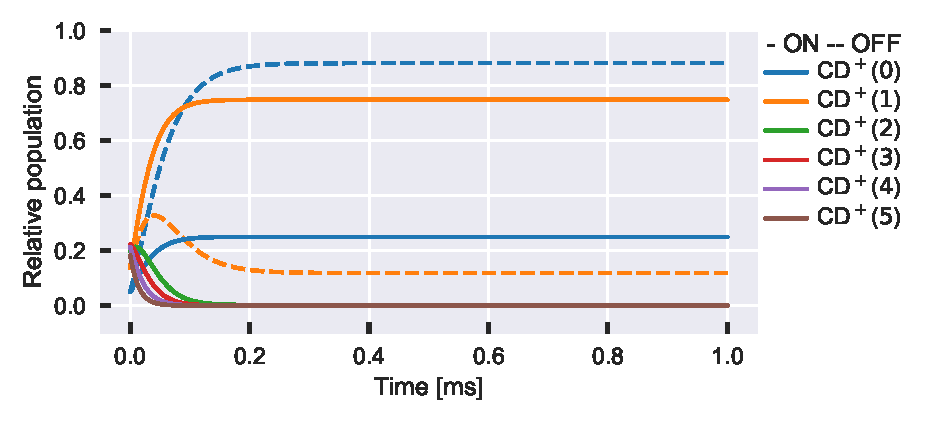
\includegraphics[width=1\textwidth]{figures/simulations/coll_rad/CD+_He_f-time__transition_0-1_0.001s_population_ratio-higher-rad.pdf}}{}{\label{fig:ROSAA-sim-coll-rad-population-higher-rad}}
    \hfill
    \Subfigure[0.49]{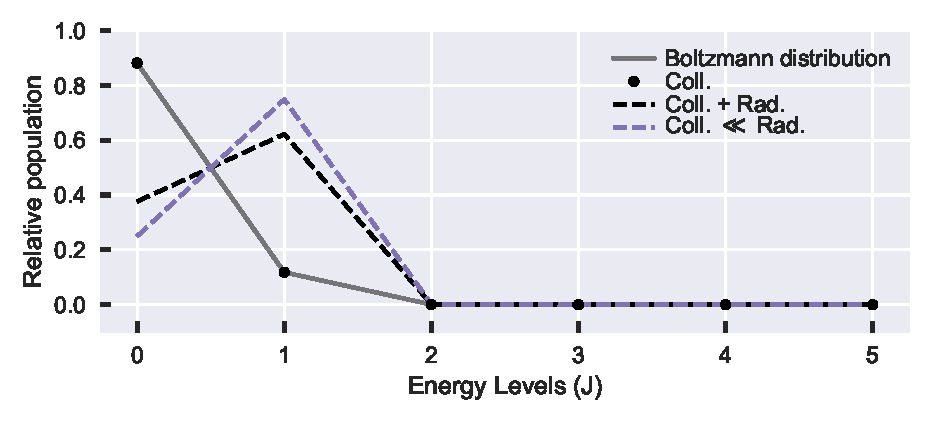
\includegraphics[width=1\textwidth]{figures/simulations/coll_rad/CD+_He_f-time__transition_0-1_0.001s_boltzman_comparision-higher-rad.pdf}}{}{\label{fig:ROSAA-sim-coll-rad-boltzmann-higher-rad}}
    
    \caption{(a) Simulated relative rotational level populations for \CD and corresponding number $J$ levels as labelled in parenthesis. The population evolves from $t=0$ (T$_{coll}=300$ K) to reach equilibrium at $t<0.5$ ms. The solid and dashed lineshapes correspond with (ON) and without (OFF) the presence of radiation on the \CD \CDline transition. The radiation power is 3.5 W. (b) Compares the Boltzmann distribution at 7 K with the relative population involving only collisional process (Coll.), collision and radiative process for power $3.5\ \mu$W (Coll. + Rad.), and collision and radiative process for power 3.5 W (Coll. $\ll$ Rad.), at $t=1$ ms.}
    \label{fig:ROSAA-sim-coll-rad-population-boltzmann-higher-rad}
\end{figure}